\section{Modeling issues}
Modeling an algorithm is a complex task which involves measuring memory requirements, program size, power consumption but most of all computational time: comparisons, multiplications and hard disk accesses.

Measurements are taken according to theoretical analysis in a specific model of computation, giving asymptotic (lower) bounds typically focusing on the worst case. 

Bounds are usually given by a function $f : \mathbb{N} : \mathbb{N}$ that maps input length to running time. The input length may be the size of the input in bits or the number of arguments, or just the number of arguments.

Performance can be measured calculating running time and storage space, or according to number of basic operations - easier but with less meaningful results.

\subsection{Models of computation}
The Touring machine is a simple model, allowing to alter the current memory location and useful to discuss computability. It is not a good model to develop efficient algorithms.

RAM has an input and an output tape, with infinite but countable number of registers holding indirectly addressed integers. Operations:
\begin{itemize}
	\item Input operations (read);
	\item Output operations (write);
	\item Register-register transfers;
	\item Indirect addressing (loading content of the $i$-th register to the $j$-th);
	\item Branch based on comparisons;
	\item Jump to position $x$;
	\item Arithmetic instructions.
\end{itemize}
The cost model is uniform (every operation takes time 1) or logarithmic (depending on the content of the cells). The largest value stored in a bounded word model may not exceed $2^\omega$, where usually $\omega = \log_2 n$.

\subsection{Complexity bounds and asymptotic notation}
There are different types of complexity bounds:
\begin{itemize}
	\item Best-case: $C_{bc}(n) := min\{C(x) | \abs{x} = n\}$;
	\item Worst-case: $C_{wc}(n) := max\{C(x) | \abs{x} = n\}$;
	\item Average (expected) case: $C_{avg}(n) := \frac{1}{\abs{I_n}} \sum_{\abs{x} = n} C(x)$ \\
	$C_{avg}(n) := \sum_{x \in I_n} \mu(x) C(x)$.
\end{itemize}
$I_n$ is a set of instances of length $n$.

There also are amortized complexity, the average cost of data structure operations over a worst case sequence, and randomized complexity (non-deterministic algorithms), worst case using random bits for a fixed input. Randomized complexity has cost $C(x)$ as expected cost $E[C(x)]$.

Running times are interesting for large values of $n$, without considering constant additive terms and exact numbers. A linear speed-up is always possible, but the complexity should be expressed by simple (positive, from $\mathbb{N}$ to $\mathbb{R}^+$) functions.
$$O(f) = \{g\ |\ \exists c > 0\ \exists n_0 \in \mathbb{N}_0\ \forall n \geq n_0 : [g(n) \leq c \cdot f(n)]\} \qquad g(x) \in O(f): 0 \leq \lim\limits_{n \rightarrow \infty} \frac{g(n)}{f(n)} < \infty$$
$$\Omega(f) = \{g\ |\ \exists c > 0\ \exists n_0 \in \mathbb{N}_0\ \forall n \geq n_0 : [g(n) \geq c \cdot f(n)]\} \qquad g(x) \in \Omega(f): 0 < \lim\limits_{n \rightarrow \infty} \frac{g(n)}{f(n)} \leq \infty$$
$$\Theta(f) = \Omega(f) \cap O(f) \qquad g(x) \in \Theta(f): 0 < \lim\limits_{n \rightarrow \infty} \frac{g(n)}{f(n)} < \infty$$
$$o(f) = \{g\ |\ \forall c > 0\ \exists n_0 \in \mathbb{N}_0\ \forall n \geq n_0 : [g(n) \leq c \cdot f(n)]\} \qquad g(x) \in o(f): \lim\limits_{n \rightarrow \infty} \frac{g(n)}{f(n)} = 0$$
$$\omega(f) = \{g\ |\ \forall c > 0\ \exists n_0 \in \mathbb{N}_0\ \forall n \geq n_0 : [g(n) \geq c \cdot f(n)]\} \qquad g(x) \in \omega(f): \lim\limits_{n \rightarrow \infty} \frac{g(n)}{f(n)} = \infty$$
It is important to note that a function belongs to a set, does not equal to it. The constant factors can be written or ignored.

Property of linearity of sum and multiplications apply to functions with the property $\exists n_0 > 0 \forall n \geq n_0 : f(n) > 0$ for $O$ and $\Theta$.

Asymptotic notations must not be used within induction proofs: for any constants $a, b, \log_a n = \Theta(\log_b n)$ and the base can be ignored. In general, $\log n = \log_2 n$.

Sometimes the input of an algorithm consists in several variables, which extend the general definition of asymptotic notation

\section{Recurrences}
Recurrences need to be solved to bring the expression from the number of comparisons to the closed form. This can be done in several ways:
\begin{enumerate}
	\item Induction, proving or disproving the solution is correct by taking a wild guess of it (assuming $n$ respects certain conditions, such as being a power of 2 to apply the logarithm);
	\item Master Theorem, obtaining tight asymptotic bounds applicable to most recurrences;
	\item Characteristic Polynomial, to solve linear homogeneous recurrences;
	\item Generating Functions, a more general technique also for non linear relations;
	\item Transformation of the Recurrence to a linear one.
\end{enumerate}

\subsection{Master theorem}
Let $a \geq 1$, $b \geq 1$ (usually strictly larger) and $\epsilon > 0$ denote constants. Considering the recurrence
$$T(n) = aT\Big( \frac{n}{b} = f(n) \Big)$$
where the first term can be substituted with a constant $c$ havig $n$ sufficiently small, there are three possible cases:
$$f(n) = O(n^{\log_b(a) - \epsilon}) \implies T(n) = \Theta(n^{log_ba})$$
$$f(n) = \Theta(n^{\log_b(a)}\log^kn) \implies T(n) = \Theta(n^{\log_ba}\log{k+1}n) \quad k \geq 0$$
$$f(n) = \Omega(n^{\log_b(a) - \epsilon}) \land af\Big( \frac{n}{b} \Big) \leq cf(n) \text{ for sufficiently large \textit{n} and $c < 1$} \implies T(n) = \Theta(f(n))$$ 
This methods divides the problem in $a$ sub-problems of the same size \nicefrac{n}{b} and then combines them. The master theorem can be applied looking at the function $f(n)$ and comparing it to $n^{\log_ba}$ to understand which case it falls into:
\begin{enumerate}
	\item Strictly smaller;
	\item Same growth, adding a logarithm factor with increasing exponent;
	\item Bigger growth (usually not happening with good recursive algorithms);
	\item None of those cases (theorem invalid).
\end{enumerate}

The Master theorem can be proven using a recursion tree to visualize the running time of an algorithm, assuming $n$ is in the case $b^l$ with non-recursive case applied to problem of the size 1. 

\begin{figure}[h]
	\centering
	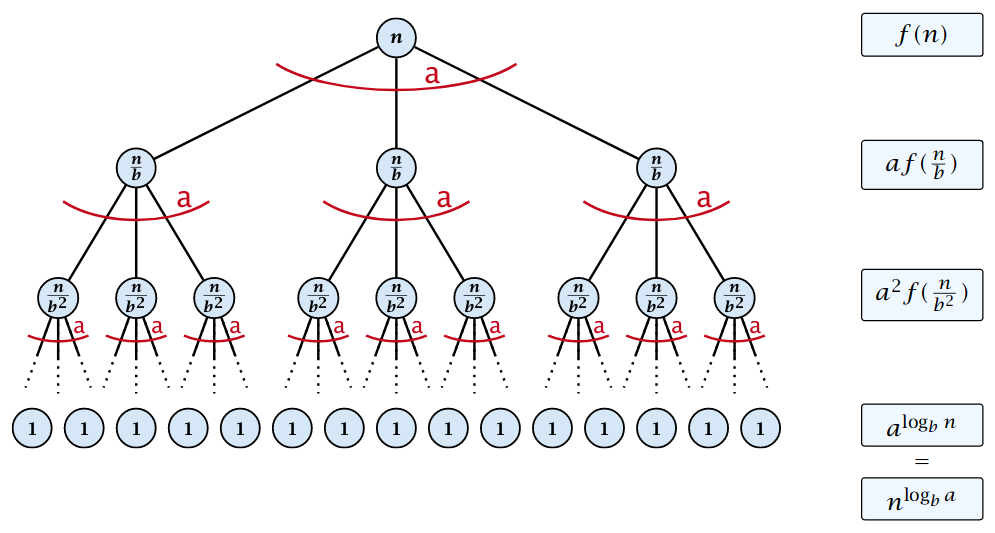
\includegraphics[scale=0.43]{lectures/images/master_tree.png}
\end{figure}

The tree stops when timing becomes $a^{log_bn}$, ignoring smaller sub-problems. From this can be derived the final equation, assuming $(b^{log_ba})^{log_bn} = a^{log_bn} = n^{log_ba} = (b^{log_bn})^{log_ba}$.

$f(n)$ (the cost of the algorithm at the first step) is compared to the three cases: if it's the first (smaller), the actual computation is performed at the lower levels. If functions have the same growth, the running time is approximately the same at every level - otherwise, the total time is dominated by the root (technically, not happening in practice). 

This gives a formula which needs to be evaluated for each case: 
$$T(n) = n^{log_ba} = \sum_{i=0}^{log_bn-1}a_if \Big( \frac{n}{b_i} \Big)$$

\section{Linear recurrences}
Linear recurrences (without products of $T[n]$) are in the form:
$$c_0T(n) + c_1T(n-1) + c_2T(n-2) + \dots + c_kT(n-k) = f(n)$$
Since the Master theorem only gives asymptotic bounds on divide-et-impera problems, it gives no information on where the input starts and what actual value it assumes. The operation also differs, since it is a subtraction, and the recurrence is defined of order $k$ (constant coefficients $c_0, c_k \neq 0$). 

The general form does not depend on $n$, but only from the preceding values. If $f(n) = 0$ then the relation becomes a linear, homogeneous recurrence relation. 

The solution is completely determined by a set of boundary conditions, that specify values for $T[i]$: any  $k$ consecutive results allow to set a solution and non-consecutive numbers may not be an appropriate set of boundary conditions.

The approach consists in determining all solutions and picking the correct one based on boundaries. The solution space of $T$ (of dimension $k$) fulfilling a recurrence relation is a vector space, and satisfies the linearity properties: there exists an $\alpha$ that makes the equation equal to 0.

A non-trivial solution needs to describe the elements in a closed form, underlining how the vector space looks like while respecting boundaries. It has the form $\lambda^n, \lambda \neq 0$, meaning that the sequence of every element $c_i$ multiplied by $\lambda^{n-i}$ is equal to 0 for all $n \geq k$.

Dividing by $\lambda^k$ gives that all the constraints are identical to:
$$c_0\lambda^k + c_1\lambda^{k-1} + \dots + c_k = 0$$
This means that if $\lambda^i$ is a root of $P[\lambda]$ then the vector $T[n] = \lambda^i_n$ is a solution to the recurrence relation. 

The polynomial can be decomposed using complex roots, which because of the linear space property still consist in a feasible solution with arbitrary values $\alpha_i$. 

Every sequence having $k$ distinct roots in the solution space can be written in the form:
$$\alpha_1\lambda^n_1 + \alpha_2\lambda^n_2 = \dots + \alpha_k\lambda^n_k = 0$$
There is one solution for every possible choice of boundary conditions, according to $\alpha_i$. 

The solution is found taking the inverse of the Vandermont matrix with column vectors $\lambda$, which are linearly independent. The determinant is computed repeating products and subtractions.

\subsection{Homogeneous case}
If roots are not all distinct (some of them have multiplicity of at least 2), then not only $\lambda_i^n$ is a solution, but also $n\lambda_i^n$. 





